\chapter{Geometry and Measurement: Part II}

The connection between solving a problem algebraically and solving it graphically is missed at times, but many problems in the SAT math section can be solved using either. Remember that to solve a system of system of equations algebraically is the same thing as looking for the point of intersection on their graphs. If, for example, you are working with two lines, and their graphs do not intersect, then the lines are parallel as in Figure \ref{fig:parallel_lines}. If the intersection of the two lines form a $90^\circ$ angle, then the lines are perpendicular as in Figure \ref{fig:perpendicular_lines}.

\bigskip
\begin{figure}[h]
\centering
\begin{minipage}[b]{0.45\textwidth}
\centering
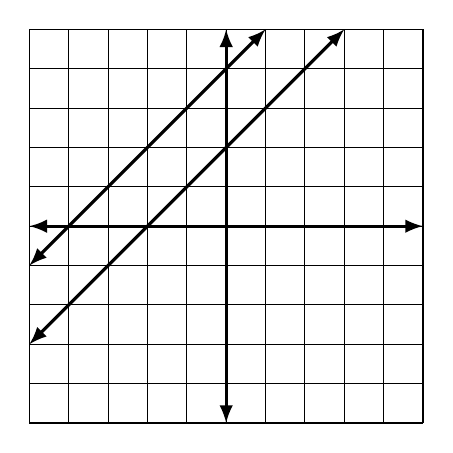
\begin{tikzpicture}[scale=0.5]
\draw (0,0) grid (10,10);
\draw[very thick, latex-latex] (0,5) -- (10,5);
\draw[very thick, latex-latex] (5,0) -- (5,10);
\draw[very thick, latex-latex] (0,2) -- (8,10);
\draw[very thick, latex-latex] (0,4) -- (6,10);
\end{tikzpicture}
\caption{Parallel lines}
\label{fig:parallel_lines}
\end{minipage}
\quad
\begin{minipage}[b]{0.45\textwidth}
\centering
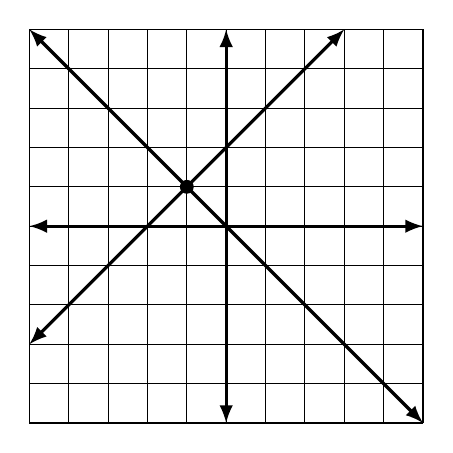
\begin{tikzpicture}[scale=0.5]
\draw (0,0) grid (10,10);
\draw[very thick, latex-latex] (0,5) -- (10,5);
\draw[very thick, latex-latex] (5,0) -- (5,10);
\draw[very thick, latex-latex] (0,2) -- (8,10);
\draw[very thick, latex-latex] (0,10) -- (10,0);
\fill (4,6) circle (5pt);
\end{tikzpicture}
\caption{Perpendicular lines}
\label{fig:perpendicular_lines}
\end{minipage}
\end{figure}